\documentclass[12pt]{article}
\input{/home/dmitry/Work/Research/thesis/FINALE/settings.tex}
\graphicspath{{/home/dmitry/Work/Research/thesis/FINALE/INTRODUCTION/content/}}

%\documentclass[PhD_Thesis.tex]{subfiles}
\begin{document}

%\section*{Abstract}
%The surface and interior wave motions interact with the sea bottom irregularities altering gravity 
%wave energy propagation. Directional scattering and mode conversion will inevitably reshape a wave 
%field and will impel restructure of localized energy budgets. Here three geophysically important 
%cases are investigated: (1) a tsunami wave scattering from a prominent sea mount, (2) origination 
%of a semidiurnal internal tide and (3) reflection of the internal tide from a continental slope. 
%These problems are investigated by means of numerical experiments and theoretical analysis.\\
%A tsunami wave is scattered by Koko Guoyt such that amplified and delayed signals were observed 
%during recent tsunami events. The numerical simulations emphasize complicated response. The energy 
%focusing occurs in dependence to tsunami incidence angel and frequencies involved. Koko guoyt as 
%having asymmetrical shape selectively amplifies tsunami wave frequency. The provided theoretical 
%analysis further outlines regions and parameters which would lead to higher amplification.\\
%Internal tides originate from surface tide interaction with steep submarine ridges. This phenomena 
%undergoes temporal variation leading to nonstationarity in the far field. It is shown for Tasman 
%Sea that remote internal tide modulates magnitude of energy conversion. Further leading to spatial 
%variability many kilometers away.\\
%The Tasman Sea internal tides impinge on the continental slope partially reflecting. The 
%reflectance markedly depends on generation of along slope leaky mode. Under some conditions 
%coupling with the surface tide occurs leading to overall energy increase (additional source?) that 
%outgoing energy becomes larger than incident amount. This deviates from classical two dimensional 
%view on reflection/scattering process of the internal tides. The presented estimates of energy 
%transfers further emphasize large variability mainly coming from along slope topography 
%inhomogeneity.\\
%Results for the problems conspicuously show importance of three dimensional topographic structure 
%in order to describe wave energy propagation. This has strong effect on variability in the 
%resulting wave field and wave energy sinks.

\newpage
\section{Introduction}
Oceanic gravity waves fundamentally contribute to the redistribution of mechanical energy in the 
world ocean. The wave energy pathways can be altered in a result of interaction with large scale 
sea bottom features such as submarine mountains, trenches and continental slopes. These processes 
shape wave propagation, cause energy dissipation and thus give rise to variation in 
the energy budgets. In this work, by means of numerical simulations, energy scattering of tsunamis 
and internal waves of tidal frequency (internal tides) is examined for realistic cases of their 
interaction with ocean's bottom relief.\\
Tsunami is a transient wave impulsively forced by submarine earthquakes. The waves traverse vast 
expanses of the oceans and encounter numerous sea bottom features \citep{mofjeld2001tsunami}. 
Such interaction with Hawaiian-Emperor seamount chain and Hess Rise diverts energy from initially 
uniform propagation \citep{kowalik2008kuril, tang2012direct}. Now wave intensity is focused 
into tight, ``pencil" beams that later lead to diverse waveforms in far-field. This is observed as 
numerous wave trains arriving in irregular sequence and with drastic changes in magnitude. For 
example, during the 2011 Tohoku-oki tsunami observations made by tidal gauges on the US West Coast 
clearly demonstrated spatial-temporal variation of tsunami surges \citep{Borrero2013} such that 
some of the largest waves unexpectedly appeared with a several hour delay after the leading wave. 
This problem is investigated in the Chapter 1. Scattering by Koko Guyot, the largest submarine 
seamount in the Emperor chain (Figure 1), is studied in order to quantify and provide description 
for the observed far-field signals during two recent tsunami events: the 2006 Kuril and 2011 
Tohoku-oki tsunamis.\\
The second problem considered here explores internal waves that pervade ocean's interior. Their 
existence owns to water column stratification since these waves manifest as an oscillatory motion 
of isopycnal surfaces. The initial perturbation can be forced by different mechanisms: wind 
stress \citep{garrett2001near}, buoyancy flux \citep{garrett1979internal}, ice ridge keels 
\citep{morison1986internal} or even tsunami \citep{santek2007satellite}. As well, tidal 
currents at steep topography brings existence of internal tides. These are baroclinic waves 
that oscillate with tidal or quasi-tidal frequency.\\
One reason to study baroclinic tides is their role in dissipation of barotropic, surface tidal 
energy \citep{munk1997once}. Current estimates suggest that 1/3 of total tidal energy is 
converted into internal motions in the deep ocean \citep{egbert2000significant}. From this roughly 
1/3 is directly lost to turbulent mixing right at generation sites \citep{st2002role} while the 
rest is emitted as freely propagating waves in form of tight beams \citep{simmons2004tidally, 
zhao2016global}. These structures are observed to cross the ocean basins without much 
attenuation. This finding fuels scientific research to understand where and how the baroclinic 
tidal energy is dissipated. Since the deposition sites primarily would occur deep below direct 
wind influence, the internal tides are thought to be a candidate for providing mechanical energy to 
close the upwelling branch of Meridional overturning circulation \citep{munk1998abyssal}. 
Regardless of global importance, the baroclinic tides are relevant for local processes such as 
water mass transformation \citep{stigebrandt1989vertical}, vertical nutrient fluxes 
\citep{sharples2007spring}, sediment \citep{hotchkiss1982internal} and larvae transports 
\citep{pineda1999circulation}.\\
All of the above is crucially dependent on internal-tide generation, propagation and scattering 
that are still poorly constrained. The Tasman Tidal Dissipation Experiment (TTIDE) had its 
goal to provide description of the internal tide reflection in relatively simple setting of Tasman 
continental slope. An internal tidal beam originated at Macquarie Ridge, New Zealand transverses 
Tasman Sea and impinges on the slope of Tasmania (Figure 1). The primary aim is to quantify amount 
of wave energy being reflected back into open sea, scattered into higher vertical modes and 
consequently, describe processes associated with sink of energy. These problems are addressed in 
Chapters 2 and 3.\\
The two geophysical problems examined in the thesis represent a wave scattering by 
inhomogeneity in propagation media. Here, it takes form of rapid change in ocean depth imposing 
constrains on fluid motion. The accompanying transfers are intrinsically linked to energy flux 
approach. This is reviewed in \textbf{Section 2} by considering a normal mode dynamics, while 
\textbf{Section 3} describes energy characteristics associated with wave transformations caused by 
interaction with bathymetry.\\

%physically based mixing parametrization

%Consequently, this provides insight for future parametrization 
%of internal tide reflection that would allow for energetically constrained internal wave 
%models (e.g. \citep{eden2014energy}.

%\textit{At such location the energy would drain into perturbations of isopycnals that further can travel hundreds of  leagues without any significant loss of energy. In the second part of my thesis origination, propagation and dissipation of the internal tidal beam is investigated on the example of Tasman Sea.\\
%A global internal tide model, satellite altimetry measurements and in situ observations indicate that a ridge south of New Zealand is a site for the generation of the strong tidal beam that is directed towards the Tasman Shelf break. The low mode internal wave beam undergoes scattering from topography, which transfers energy to shorter length scales. Thus, understanding of local energy processes will lead to a more detailed picture of tidal energy dissipation.\\
%\textbf{PLUGIN: 2 TW, 1 TW, Macquarie Ridge, internal tides produce transport of particulates: sediments and can cause strong currents in deep ocean. Role in tidal dissipation, Internal tides what became apparent recently are important energy transporters.}

\newpage

\section{Normal modes in flat-bottom sea}
Tsunami and internal tides are a case of long gravity waves. Their typical wavelengths are order of 
100 km being larger than the ocean's mean depth. So the wave dynamics can be well described in 
linear, hydrostatic framework. As first step, the wave propagation is discussed for flat-bottom 
ocean. The equations of motion in stratified, Boussinesq ocean on an f-plane 
\citep{kundu2008fluid, cushman2011introduction} will take mathematical form of,
\begin{align}
\label{In:Beq}
\pder[u]{t} - f v = -\frac{1}{\ib{\rho}_0}\pder[p]{x}\\
\pder[v]{t} + f u = -\frac{1}{\ib{\rho}_0}\pder[p]{y}\\
0 = -\pder[p]{z} - \rho g\\
N^2 w = -\frac{1}{\ib{\rho}_0} \pderr[p]{z}{t}\\
\pder[u]{x} + \pder[v]{y} + \pder[w]{z} = 0
\end{align}
with $(u,~v,~w)$ being velocity along zonal, meridional and vertical axis, $f$ - Coriolis parameter, $p$ - perturbation pressure arising either from sea level oscillations or isopycnal displacements within stratified water column given by Brunt-Vaisala frequency $N^2 = -\frac{g}{\ib{\rho}_0}\pder[\rho_0]{z}$. Additionally, boundary conditions are imposed on the surface and bottom,
\begin{align}
w|_{z = 0} = \pder[\zeta]{t},~p|_{z = 0} = \ib{\rho}_0 g \zeta\\
w|_{z = -H} = 0\label{In:bc.swe}
\end{align}
The both conditions are of linear form since the sea level motions are much smaller than the 
acceleration due to gravity, and the ocean depth is fixed. Such formulated problem allows 
separation of vertical motions by employing following decomposition,
\begin{align}
(u, v, p)(x,y,z,t) = \sum_{n = 0} [u_n(x,y,t), v_n(x,y,t), p_n(x,y,t)]\psi_n(z)\\
w(x,y,z,t) = \sum_{n = 0} [w_n(x,y,t)] \int_{-H}^z \psi_n(z) dz\\
\rho(x,y,z,t) = \sum_{n = 0} [\rho_n(x,y,t)] \frac{d \psi_n(z)}{dz}
\end{align}
Upon substitution Sturm-Liouville problem is obtained for vertical structure (basis) functions 
$\psi_n(z)$\footnote{note this is for horizontal variables, usually it is written for vertical 
velocity since boundary conditions are expressed right away},
%\pder[\frac{1}{N^2 - \omega^2} \pder[\psi_n]{z}]{z} + \big(1 - \frac{f^2}{\omega^2} \big) \frac{\psi_n}{c^2_n} = 0
\begin{equation}
\frac{d}{dz}\big( \frac{1}{N^2} \frac{d \psi_n}{dz} \big) + \frac{1}{c^2_n}\psi_n = 0
\end{equation}
with an eigenvalue for a respective $n$-th vertical mode given by $c_n$. This is a phase speed in 
non-rotating ocean with an equivalent depth, $D_n$ such that $\sqrt{g D_n} = c_n$. The carried out 
decomposition detaches vertical motions from horizontal dynamics reducing the initial set 
\eqref{In:Beq} to Laplace tidal equations,
\begin{subequations}
\label{In:sweq}
\begin{align}
%\begin{split}
\pder[\vec{u}_n]{t} + f \vec{k} \times \vec{u}_n = -\frac{1}{\rho_0} \nabla p_n \label{In:swe.mom}\\
\frac{1}{\rho_0} \pder[p_n]{t} + g D_n \nabla  \cdot \vec{u}_n = 0 \label{In:swe.cont}
%\end{split}
\end{align}
\end{subequations}
This states dynamical equivalence between barotropic, surface  wave and baroclinic, internal waves 
if the ocean stratification would be absent and the apparent depth would be $D_n$. In actuality, 
$0$-th mode represents a barotropic solution with vertically uniform dynamics ($\psi_0 = const$) 
and the equivalent depth $D_0 \simeq H$ \citep{hendershott1981long}. This mode resembles pure 
surface wave propagation such as in tsunami wave problem. The infinite sequence of higher vertical 
modes are internal modes that produce negligible sea level perturbations. This allows complete 
separation between barotropic and baroclinic motions which is similar to imposing rigid lid 
condition on internal modes \citep{kundu2008fluid}.\\
The main interest is in linear wave phenomena, so harmonic temporal behavior $e^{i \omega t}$ will be implied leading to Helmholtz equation,
\begin{align}
\label{In:helmeq}
(\omega^2 - f^2) p_n + c_n^2 \Delta p_n = 0
\end{align}
Making a plane wave ansatz, $e^{-i\vec{k} \cdot \vec{x}}$, currents and pressure will be related as
\begin{align}
\begin{split}
p_n = p_{0n} e^{i (\omega t - \vec{k} \cdot \vec{x})}\\
u_n = \frac{1}{\ib{\rho}_0} \frac{\omega k_x + i f k_y}{\omega^2 - f^2} p_n\\
v_n = \frac{1}{\ib{\rho}_0} \frac{\omega k_y - i f k_x}{\omega^2 - f^2} p_n
\end{split}
\end{align}
Than from \eqref{In:swe.cont}, a dispersion relation for Sverdrup waves follows,
\begin{equation}
\omega^2 = f^2 + c^2_n |\vec{k}|^2
\end{equation}
The waves are dispersive as a result of Earth's rotation with phase and group speeds are
\begin{align}
c_{p} = (1 - \frac{f^2}{\omega^2})^{-1/2} c_n,~c_g = (1 - \frac{f^2}{\omega^2})^{1/2} c_n,~c_p c_g 
= c_n^2
\end{align}
For the most energetic mode-1 semidiurnal internal tide, phase travels with speed of $4~m/s$, but 
group speed is only $2~m/s$. So slow traveling wave is inevitably affected by background 
oceanic circulation. On contrary, tsunami waves exhibit shallow-water, nondispersive behavior with 
phase and group speeds of $\sim O(100~m/s)$ owing to small periods in comparison to inertial 
period. Tsunami waves cross ocean basins in a matter of hours without any appreciable 
interaction with ocean's dynamical state.\\~\\
In deep ocean, where bottom's topography does not demonstrate large spatial gradients, normal 
modes are an useful approach in description of wave-intensity changes. In order to do so energy 
equation can be developed from \eqref{In:sweq}. Multiplying momentum equations by $\vec{u}_n$ and 
continuity equation by $p_n$, adding both expressions and depth integrating one obtains
\begin{equation}
(E_k + E_p)_t + \nabla \cdot \vec{F} = 0 \label{In:eneq}
\end{equation}
Additionally, depth averaging is carried out so that energy flux will be defined,
\begin{equation}
\vec{F}_n = \frac{1}{H} \vec{u}_n(t) p_n(t) \int_{-H}^0 \psi^2(z) dz \label{In:fldef}
\end{equation}
For tsunami wave propagation due to their barotropic nature $\psi(z) = const$ and $p_n = \rho_0 g 
\eta$, the expression takes its classical form for surface wave propagation 
\citep{henry2001representation}, $\vec{F} = \rho_0 g \vec{u} \zeta$.\\
In internal tide studies period averaging further simplifies calculations,
\begin{align}
\vec{F}_n = \frac{1}{2} \cj{\vec{u}}_n p_n \int_{-H}^0 \psi^2(z) dz
\end{align}
where velocity and baroclinic pressure are now complex amplitudes of harmonic fit and $\cj{}$ is a 
complex conjugate.\\
The obtained expressions for energy flux comprises only pressure-work term, i.e. transport of 
energy is dictated by pressure forces. In full formulation this is augmented with nonlinear 
contributions made by advection and dissipative forces \citep{gill2016atmosphere}. These terms 
are negligible presuming deep ocean propagation where the wave's spatial dimensions are large and 
magnitude of dynamical variables is small.\\
%\citep{kang2012energetics}, \citep{nash2012unpredictable}
Away from scattering region, an energy budget could be constructed following the linearized normal 
mode dynamics. Any loss in intensity of primary wave has to be balanced by energy scattered into 
other 
wave motions and by dissipative losses. The latter is not discussed here and thought to be 
comprised by residue terms. While the scattered wave field, reflected components and intermodal 
conversion are the main topic of investigation. The quantitative aspects are discussed in 
\textbf{Section 3}.\\

\section{Oceanic wave scattering}
The normal mode approach was formulated under the assumption of flat bottom with a simplified 
boundary condition, $w|_{z = -H} = 0$ that allows separation of variables. Thence, 
vertical motions are decoupled from horizontal dynamics. As a wave encounters an inclined 
slope the simplified relation does not hold and the bottom boundary condition becomes nonlinear,
\begin{equation}
( \vec{u} \cdot \nabla h )|_{z = -h(x, y)} = 0~\text{or}~w = - \vec{u}_h \cdot \nabla h 
\label{In:bcnon} 
\end{equation}
The condition states that there is no mass transport across an impermeable bottom. The wave motion 
cannot alone satisfy (\ref{In:bcnon}), and a compensating flow has to develop to preserve mass. For 
the configuration when an incident wave train encounters a vertical wall in nonrotating ocean, a 
specular reflection occurs in order to fulfill the no-flow condition. Opposing fluid motions 
will be produced by a back-scattered wave.\\
An additional condition is imposed on scattered waves such that the energy vanishes with distance 
\citep{mei1989theory, morse1946methods}. The Sommerfeld radiation condition leads to  
a far-field asymptotic:
\begin{equation}
\label{In:def.scamp}
p_{scat} \sim \frac{e^{i \vec{k} \cdot \vec{x}}}{|\vec{x}|} \Phi_s (\theta)
\end{equation}
This is an assertion for circularly spreading waves having some angular distribution $\Phi_s$, 
called a scattering amplitude. The squared quantity will furnish amount of scattered radiation. In 
the problem of tsunami-topography interaction, far-field signals could be approximated with the 
above distributions; while in internal tide reflection problem, large distances away (when 
continental slope becomes a point) an angularly integrated scattered amplitude will be directly 
related to a reflection coefficient, though wave spreading with distance has to be factored in.\\
In the near-field, a scattered wave field can be decomposed by Fourier transform whereby each 
wavenumber can be regarded as a separate component. As it propagates away, it will begin to 
separate from others. Magnitude modulations due to interference \footnote{more appropriate to say 
diffraction} will subdue. And at large distances, respective Fourier coefficient will represent a 
scattering amplitude in direction corresponding to the wave vector. As a result, Fourier transform 
depicts the far-field's distribution of energy.\footnote{ This is a fundamental idea in acoustic 
holography \citep{williams1999fourier}, should I cite other fields?.}\\
In addition to angular scattering, there could occur a transfer of energy into different vertical 
modes. Let us consider a long wave that obeys Laplace tidal equations entering a region where 
bottom slope is inclined and the full boundary condition \eqref{In:bcnon} has to be satisfied. It 
only can be fulfilled if there is a vertical velocity. A normal mode by itself is not able to 
represent the dynamics since the vertical derivative, by definition, is zero on the boundary. 
However, a superposition of modes can force horizontal convergence to cancel out the vertical 
velocity. Physically, pressure gradients should develop by displacing isopycnal surfaces which 
further radiate energy away in the form of baroclinic modes. In general, this describes a 
coupled-mode approach \citep{griffiths2007internal}. Locally-flat normal modes counteract one 
another through the boundary condition. The spatial gradients will dictate mode's magnitude to 
equilibrate the balance. Dynamically, Laplace tidal equation for each separate mode will embrace an 
additional force represented as intermodal-coupling term \citep{griffiths2007internal, 
kelly2016coupled}.\\
The intermodal conversion and energy flux carried by modes can be estimated as work done by 
vertical velocity against modal pressure, $W_{m \to n} \sim (w_{m,~scat}~p_n)|_{z = 
-h} = -((\vec{u}_m \cdot \nabla h) p_n)|_{z = -h}$. But total conversion must as well account for 
the opposite energy transfer, from $n$ to $m$, hence,
\begin{align}
\label{In:en.trans}
C_{m \to n} = -((\vec{u}_m \cdot \nabla h)~p_n)|_{z = -h} + ((\vec{u}_n \cdot \nabla h)~p_m)|_{z = 
-h}
\end{align}
Internal tide excitation can be viewed as scattering of barotropic tide by steep relief 
\citep{hendershott1981long}. If the surface tide is the $0^{th}$ mode, then energy lost can be 
diagnosed as
\begin{align}
\label{In:bt_bc}
C_{bt \to bc} = -(\vec{u}_{bt} \cdot \nabla h)~\sum_{n = 1} p_n|_{z = -h}
\end{align}
assuming that the baroclinic wave field effect on surface tide is negligible 
\citep{kelly2012cascade}. The above expression is well established in internal tide studies 
\citep{kurapov2003m, llewellyn2002conversion, pickering2015structure}.\\
For consideration of mode-1 scattering it is useful to reformulate \eqref{In:en.trans} by employing 
Leibniz's rule, the continuity equation per each normal mode, and mode's orthogonality,
\begin{align}
C_{m \to n} = \int_{-h}^{0} (u_m \nabla p_n - u_n \nabla p_m) dz
\end{align}
In the problem of internal wave propagation over uniform and gently inclined bottom 
\citep{wunsch1968propagation}, there is no intermodal conversion, $C_{m \to n} = 0$, and each 
mode's dynamics is perfectly matched by presence of others. Strictly speaking, in this case the 
wave equation is hyperbolic \footnote{(in contrary to elliptical Helmholtz equation, 
\eqref{In:helmeq})} and propagation occurs along characteristics \citep{sandstrom1969effect} or 
internal wave rays described by
\begin{equation}
\label{In:ch.angle}
\gamma = \frac{dz}{dx} = \pm \frac{\omega^2 - f^2}{N^2 - \omega^2}
\end{equation}
Slope criticality can be defined as ratio between its inclination and rays angle, $\gamma$. In 
subcritical regime of forward propagation, the ratio is less than unity. In this case for steeper 
bottom more higher modes is necessary to describe internal tide dynamics (Figure 2). Now it is 
apparent that a mode conversion will not happen, unless there is a change in topography to drive 
adjustment of mode amplitudes. On contrary, in supercritical regime, when $\nabla h > \gamma$, 
internal waves are reflected with always present generation of higher modes. Usually, they will be 
phase-locked into vertically propagating rays \citep{garrett2007internal, 
lamb2014internal} subject to breaking and dissipation \citep{lien2001observations, 
nash2004internal, klymak2011breaking}. In case of the continental slope this causes internal tide 
mode-1 reflection to decrease relative to the equivalent case of surface wave reflection.\\
As a first approximation for long waves scattering, it will be instructive to consider a problem 
with simplified geometry. This will usually consist of a step discontinuity connecting the deep 
ocean with the top of seamount (e.g. Koko Guyot) or the continental shelf. Then the boundary 
condition \eqref{In:bcnon} is analogous to fulfilling so-called matching conditions 
\citep{mei1989theory}. These are mass conservation and continuity of sea level for surface waves
\begin{align}
\vec{u}_1 h_1 = \vec{u}_2 h_2,~\zeta_1 = \zeta_2
\end{align}
In the case of internal tides - continuity of pressure and no-flow through vertical walls 
\citep{st2002role, larsen1969internal, chapman1981scattering}, the conditions are
\begin{align}
p_1 = p_2, -h_2 \leq z \leq 0 \\
\vec{u}_1 = 0, -h_1 \leq z \leq -h_2\\
\vec{u}_1 = \vec{u}_2, -h_2 \leq z \leq 0
\end{align}

\section{Organization of thesis}
The thesis consists of the following three chapters:
\begin{enumerate}
	\item[Chapter 1] makes its goal analysis of scattering of tsunami waves by Koko Guyot. The 
	approach is based on obtaining scattering amplitude \eqref{In:def.scamp}, evaluation of its 
	frequency and spatial characteristics in order to describe far-field signals. The discussion 
	and conclusions are supported with analytical calculations based on matching conditions 
	approach.
	\item[Chapter 2] deals with generation of semidiurnal internal tide at Macquarie Ridge,  
	Tasman Sea. This is studied in a detail by analysis of three dimensional structure of 
	internal wave field. The proposed mechanism explains peculiarities of conversion rates 
	\eqref{In:bt_bc}. The emitted internal tidal beam than described in the far-field with emphasis 
	on its kinematic properties.
	\item[Chapter 3] concerns the tidal beam reflection from Tasman Continental Slope. The 
	obtained energy levels show variability that is due to number of factors. Possibility of each 
	is discussed and respective estimates are made in order to propose physically reasonable 
	mechanism of internal tide dynamics in three dimensionally complex region.
\end{enumerate}
Throughout the thesis a method based on inverse modeling was used. Its mathematical rudiments are 
given in Appendix A.

\section*{Figures}
\begin{figure}
	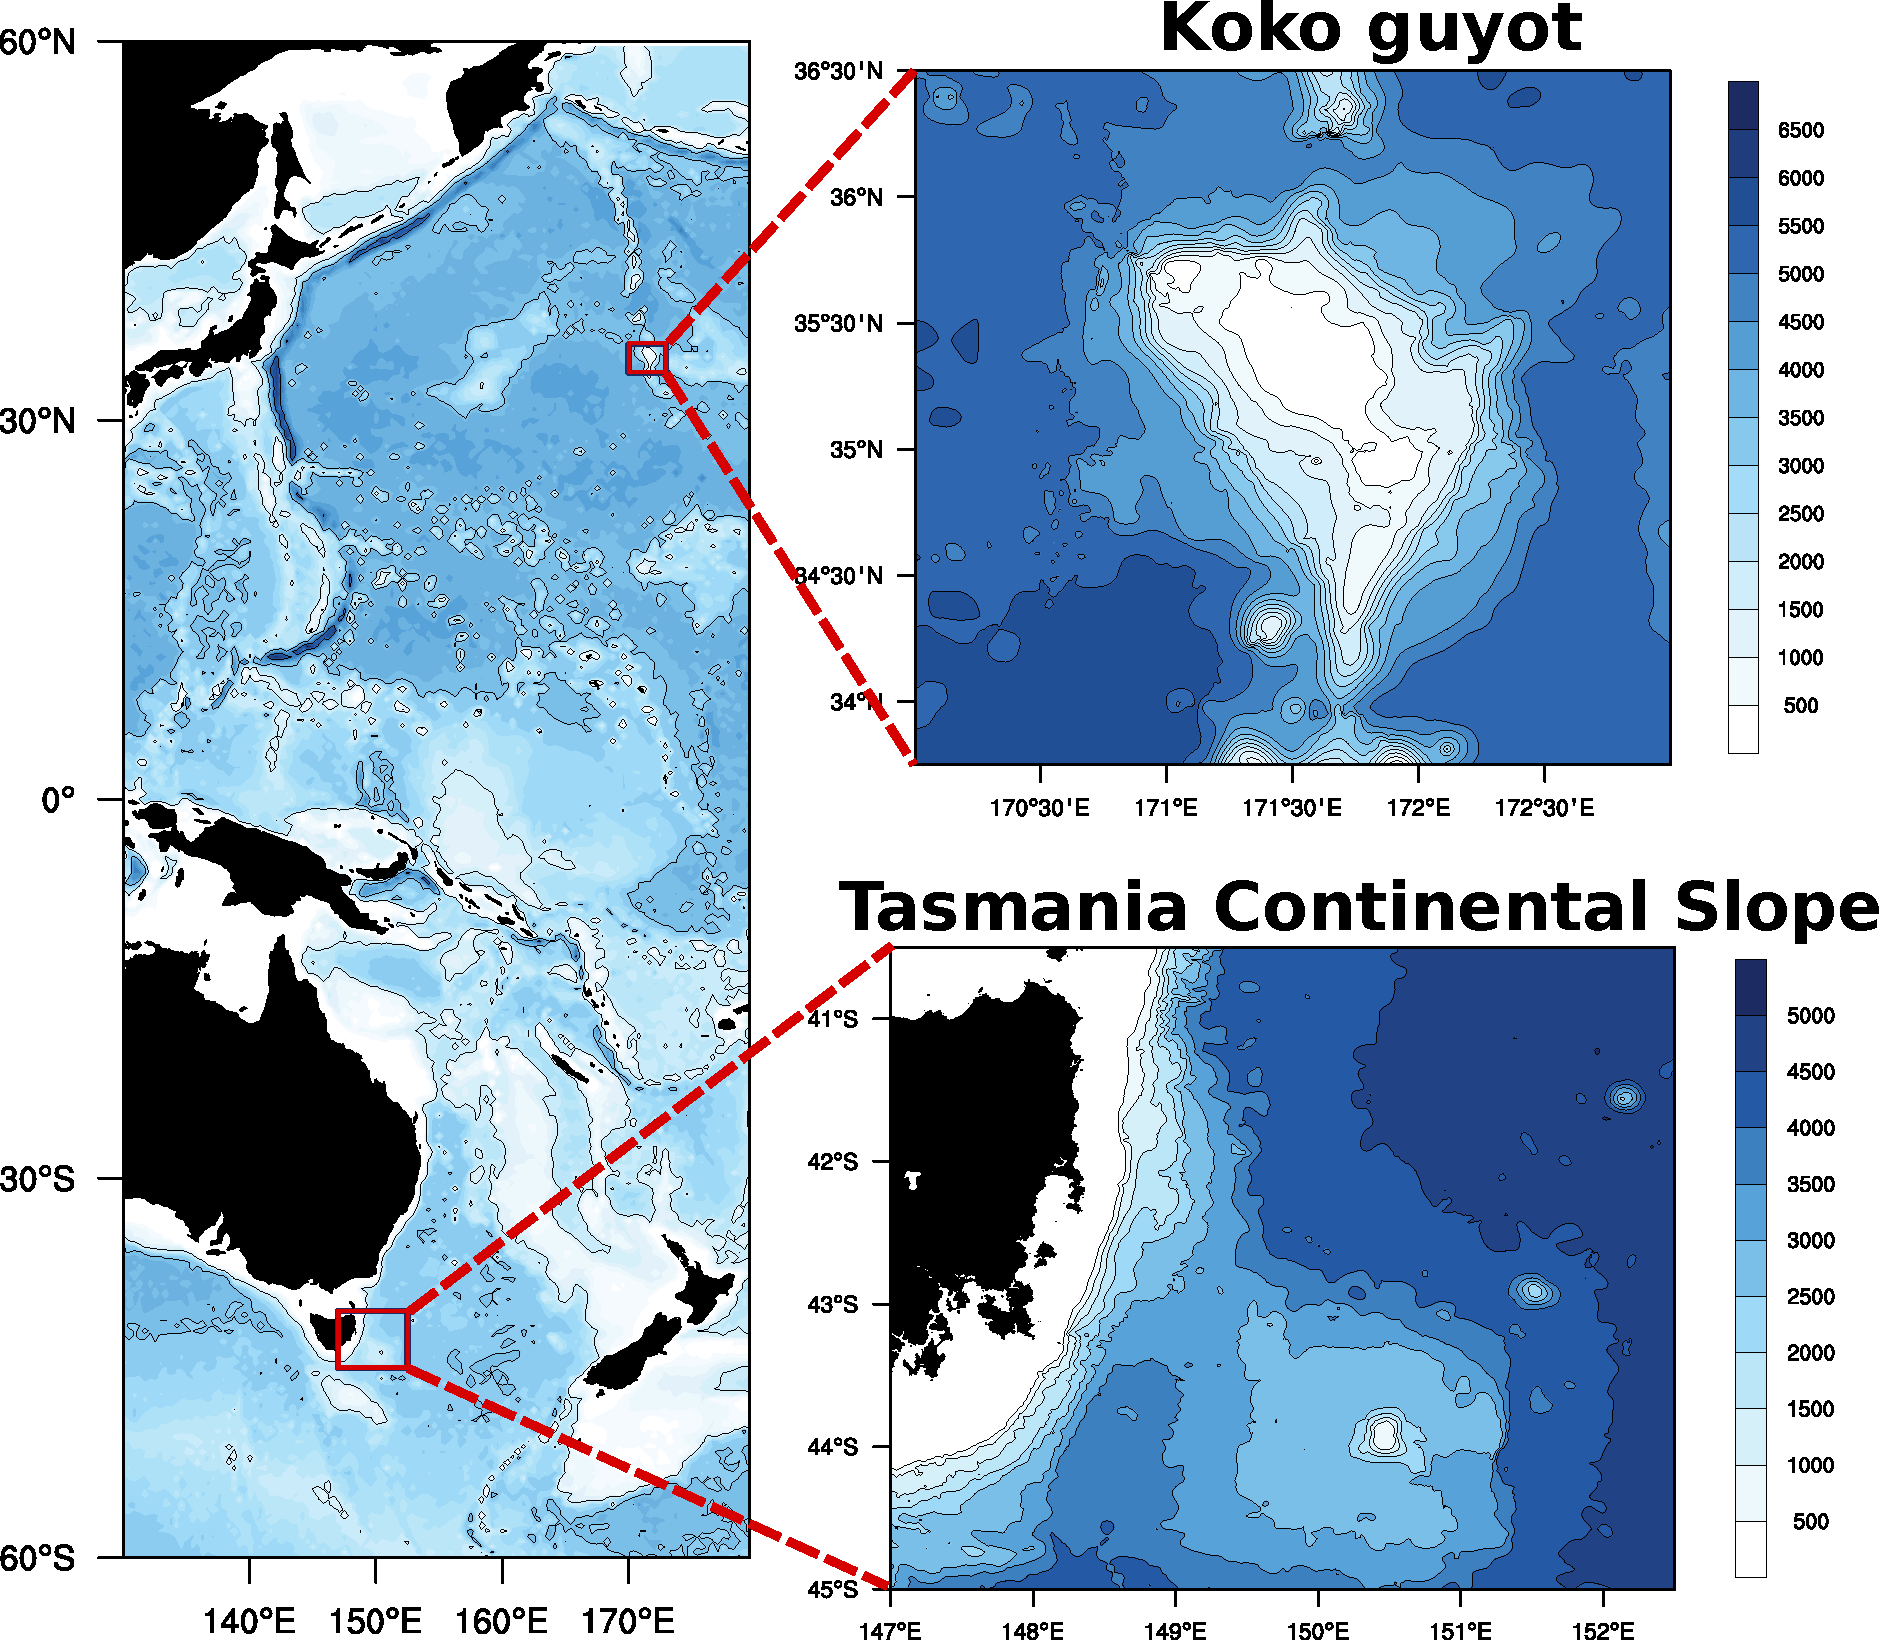
\includegraphics[scale=0.5]{/home/dmitry/Work/Research/thesis/FINALE/INTRODUCTION/figures/map_w_places.pdf}
	\caption{Bathymetric map of the Pacific Ocean with outlined regions showing geographic 
	locations of considered wave scattering problems.}
\end{figure}
	
\begin{figure}
	\includegraphics[scale=0.8]{/home/dmitry/Work/Research/thesis/FINALE/INTRODUCTION/figures/errors2.pdf}
	\caption{Error in description of internal wave structure by flat-bottom vertical modes as 
	bottom gets steeper.}
	%\includegraphics[scale=0.5]{../}
\end{figure}
%In overall, this thesis intends to investigate scattering process in three geophysical cases. In order to study this phenomena one will inevitably encounter interference which can lead to impossibility of direct energy budget estimates. Here I concerned with obtaining characteristics of how much energy was lost and how that energy was distributed in space. So decomposition of interference into elemental waves should be considered.\\
%I address this question by studying results of numerous numerical experiments with varying conditions. Hence, inconstancy of the tidal beam characteristics and its intertwine with topography and background conditions could be quantitatively described in order for better explanation of TTIDE field measurements.
% 
%\begin{enumerate}
%\item Chapter 1. Method for interference decomposition in numerical experiments on wave scattering.
%In order to quantify things such as directional distribution and reflection coefficient the field should be decomposed in order to obtain energy characteristics.
%
%\item Chapter 2. Scattering of tsunami waves by Koko Guyot.
%\item Chapter 3. Generation, structure and variability of Tasman internal tidal beam.
%\item Chapter 4. Reflection and scattering of the internal tidal beam by Tasman continental slope.
%%\item Chapter 5. Formal solution of scattering problem in framework of coupled Laplace tidal equations.
%\item Discussion, Conclusions, Future Work.
%\end{enumerate}


%occurring 
%Energy conservation, \eqref{In:eneq} sets an useful framework for analysis of the wave interaction 
%with topography. As bottom slope starts rapidly change, wave propagation undergoes variation 
%resulting in reorientation of currents, divergence in water column. But because of energy 
%conservation, amount of total energy should be preserved. Hence, energy transports of energy 
%through control volumes can present a valuable tool for description of wave interaction with 
%bottom 
%relief. The approach 
%
%I deliberately abandon nonlinear terms . Koko Guoyt depth on 
%average is around 500 m, barotropic velocity is of order $0.1~m/s$, nonlinear terms scale as $\sim 
%u^3$, while linear energy flux as $\sim g u \zeta$. It suggests that only in shallow water where 
%horizontal acceleration is of order of gravity acceleration, nonlinear terms will be a significant 
%addition to total energy transports. The same discussion on nonlinear additions stays true for 
%internal tide scattering from the Tasman continental slope which depth does not exceed $100~m$. 
%Only on shallow shelfs advection of kinetic energy becomes non-negligible 
%.\\

\newpage

\bibliographystyle{apacite}
\bibliography{/home/dmitry/Bibtex_lib/my_first_lib}

\end{document}